%%%%%%%%%%%%%%%%%%%%%%%%%%%%%%%%%%%%%%%%%
% University Assignment Title Page
% LaTeX Template
% Version 1.0 (27/12/12)
%
% This template has been downloaded from:
% http://www.LaTeXTemplates.com
%
% Original author:
% WikiBooks (http://en.wikibooks.org/wiki/LaTeX/Title_Creation)
%
% License:
% CC BY-NC-SA 3.0 (http://creativecommons.org/licenses/by-nc-sa/3.0/)
%
% Instructions for using this template:
% This title page is capable of being compiled as is. This is not useful for
% including it in another document. To do this, you have two options:
%
% 1) Copy/paste everything between \begin{document} and \end{document}
% starting at \begin{titlepage} and paste this into another LaTeX file where you
% want your title page.
% OR
% 2) Remove everything outside the \begin{titlepage} and \end{titlepage} and
% move this file to the same directory as the LaTeX file you wish to add it to.
% Then add \documentclass[12pt]{article}
\usepackage[english]{babel}
\usepackage{amsmath}
\usepackage{graphicx}
\usepackage{textcomp}
\usepackage{parskip}
\usepackage[colorinlistoftodos]{todonotes}
\usepackage{csquotes}
\usepackage{float}
\usepackage[backend=biber,style=ieee]{biblatex}
\addbibresource{bibliography.bib}

\begin{document}

\begin{titlepage}

\newcommand{\HRule}{\rule{\linewidth}{0.5mm}}
\center 

\textsc{\LARGE Iowa State University }\\[1.5cm] 
\textsc{\Large Center for Statistics and Applications in Forensic
Evidence
}\\[0.5cm] 

\HRule \\[0.4cm]
{ \huge \bfseries Shoe Print Data Collection: Additional Methods }\\[0.4cm] 
\HRule \\[1.5cm]



\begin{center}
\centering
 
\includegraphics[scale=.4]{csafe-logo}\\[1cm]
\end{center}







\end{titlepage}

\section{Introduction}

 When developing the methodology for the longitudinal shoe study conducted by the Center for Statistics and Applications in Forensic Evidence (CSAFE), collection procedures were designed to obtain the most ideal shoe-sole impression possible. While these images will be useful to the researcher and practitioner communities, they do not provide realistic examples of prints that would be collected from a crime scene/suspected crime scene. For this reason, CSAFE researchers have compiled this manual which contains procedures for further data collection and offers new, or edited, procedures that better represent the practices of current forensic examiners and crime scene teams. If at any time there is a question on any of these procedures, please make a note using a post-it note and e-mail the principal investigator, the project manager, the faculty in charge of the study, or the author of the specific procedure. 

\end{document} to your LaTeX file where you want your
% title page.
%
%%%%%%%%%%%%%%%%%%%%%%%%%%%%%%%%%%%%%%%%%
%\title{Title page with logo}
%----------------------------------------------------------------------------------------
%	PACKAGES AND OTHER DOCUMENT CONFIGURATIONS
%----------------------------------------------------------------------------------------

\documentclass[12pt]{article}
\usepackage[english]{babel}
\usepackage[utf8x]{inputenc}
\usepackage{amsmath}
\usepackage{graphicx}
\usepackage[colorinlistoftodos]{todonotes}

\begin{document}

\begin{titlepage}

\newcommand{\HRule}{\rule{\linewidth}{0.5mm}} % Defines a new command for the horizontal lines, change thickness here

\center % Center everything on the page

%----------------------------------------------------------------------------------------
%	HEADING SECTIONS
%----------------------------------------------------------------------------------------

\textsc{\LARGE Iowa State University}\\[1.5cm] % Iowa State University
\textsc{\Large CSAFE}\\[0.5cm] % CSAFE
\textsc{\large Center for Statistics and Applications in Forensic Evidence }\\[0.5cm] % Center for Statistics and Applications in Forensic Evidence

%----------------------------------------------------------------------------------------
%	2D Shoe Scanner Procedure
%----------------------------------------------------------------------------------------

\HRule \\[0.4cm]
{ \huge \bfseries EinScan Pro+ 3D Scanner: Procedure  }\\[0.4cm] % Title of your document
\HRule \\[1.5cm]

%----------------------------------------------------------------------------------------
%	AUTHOR SECTION
%----------------------------------------------------------------------------------------

\begin{minipage}{0.4\textwidth}
\begin{flushleft} \large
\emph{Author:}\\
  James E. Kruse,  \textsc{Jessica Hanrahan} % James E. Kruse
\end{flushleft}
\end{minipage}
~
\begin{minipage}{0.4\textwidth}
\begin{flushright} \large
\emph{Supervisor:} \\
Dr. Guillermo \textsc{Basulto-Elias} % Supervisor's Name
\end{flushright}
\end{minipage}\\[2cm]

% If you don't want a supervisor, uncomment the two lines below and remove the section above
%\Large \emph{Author:}\\
%John \textsc{Smith}\\[3cm] % Your name
%----------------------------------------------------------------------------------------
%	LOGO SECTION
%----------------------------------------------------------------------------------------

\includegraphics[scale=.5]{Logo}\\[1cm]

\begin{center}
\begin{tabular}{ c   |   c }

\end{tabular}
\end{center}
%----------------------------------------------------------------------------------------
%	DATE SECTION
%----------------------------------------------------------------------------------------

{\large \today}\\[2cm] % Date, change the \today to a set date if you want to be precise


%----------------------------------------------------------------------------------------

\vfill % Fill the rest of the page with whitespace

\end{titlepage}




\section{Introduction}

The following is the recommended procedure for using the EINSCAN Pro+ 3D scanner (Figure 1). While it is not the primary purpose of this devise, it will be used to create 3D, digital models of shoe soles.

\begin{figure}[!htp]
\centering
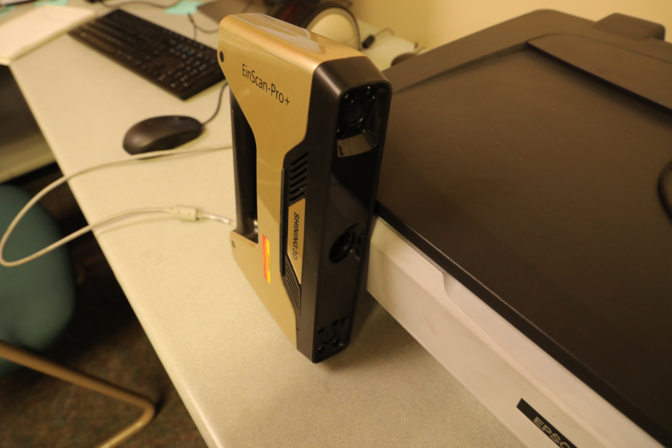
\includegraphics[scale=0.5]{3D_Scanner}
\caption{The EINSCAN Pro+ hand held 3D scanner}
\label{Image 1}
\end{figure}

\subsection{Procedure}

1.	Prior to use, contact IT to install the necessary software in the desired computer. Make sure all cords for the EINSCAN Pro+ are connected to both the scanner itself and to the computer. There will be a gray USB that will connect directly into the computer and a black power chord that will plug into the hub on the USB. This black cord will provide power to the scanner.

2. Launch the EinScan Pro program, located on the desktop. Select EinScan Pro+. Select Handheld Rapid Scan mode and create a new project. Select Non-Texture Scan, Markers/Features, and High Detail. Finish by selecting "Apply".

3. Open the shoe naming app and use the criteria located in the introduction to this manual when naming all completed files.

4. the Technition will then place a shoe on the shoe stand (Figure 2) and the stand on the floor next to their chair. If the technition wishes to stand, the shoe stand can be placed on a desk as long as no other items that could show up in the scan are near by.


\begin{figure}[!htp]
\centering
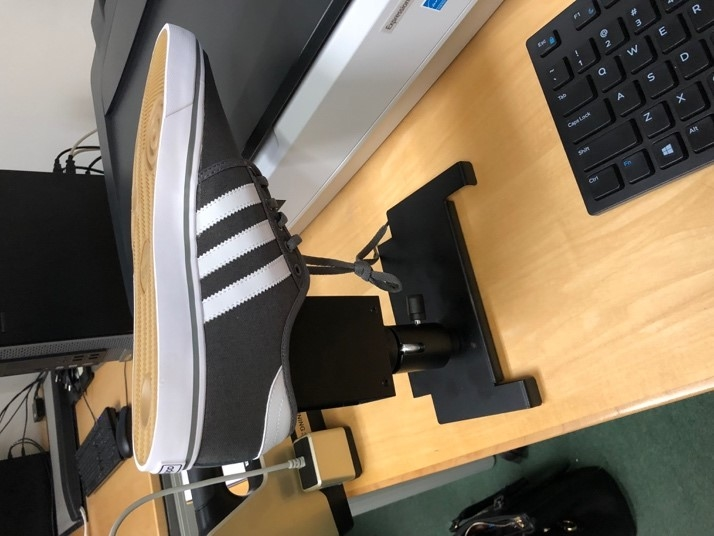
\includegraphics[scale=1, angle=270]{3D_Shoe_on_Stand}
\caption{An Adidas Shoe positioned on a shoe stand.}
\label{Image 2}
\end{figure}

5. Hold the scanner parallel to the shoe and about 12 inches above the sole (Figure 3). To begin scanning, press the play button on the scanner (Figure 4) to preview. Press play again to start scanning.

\begin{figure}[!htp]
\centering
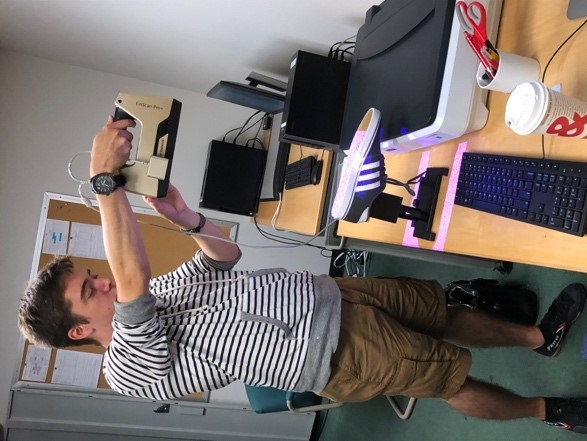
\includegraphics[scale=1, angle=270]{3D_in_use}
\caption{Technion holding the 3D Scanner in the correct position to begin the scanning process}
\label{Image 3}
\end{figure}

\begin{figure}[!htp]
\centering
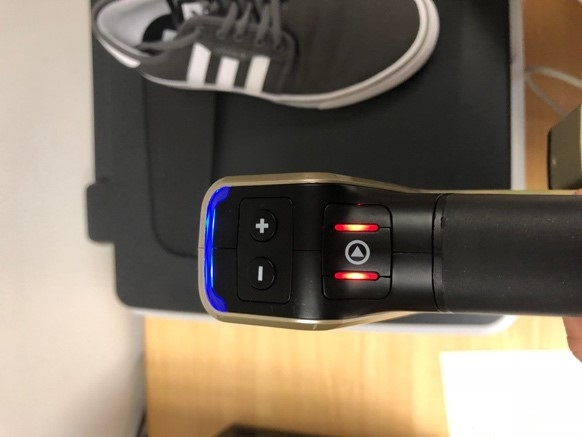
\includegraphics[scale=1, angle=270]{3D_Start_Button}
\caption{The controls for the 3D scanner. The Start button is the lower, large icon.}
\label{Image 4}
\end{figure}

\newpage

6. Start moving the scanner, slowly, from the toe of the shoe to the heel and back to the toe. Make sure to maintain, approximately, a distance of one foot from the sole.

7. The speckled red lights in the top left corner of the screen indicate areas that are not being captured well due to brightness (Figure 5). There are two ways to adjust brightness and collect more detail from each shoe sole.

\begin{figure}[!htp]
\centering
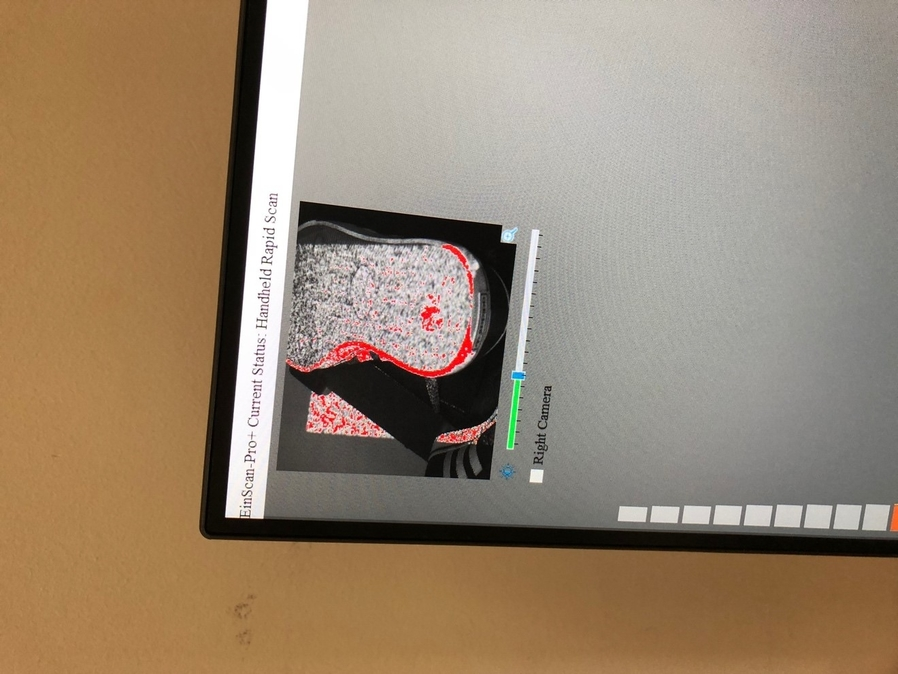
\includegraphics[scale=.75, angle=270]{3D_Brightness}
\caption{The brightness level of the scanner can be seen in this small sub-screen.}
\label{Image 5}
\end{figure}

\begin{description}
 \item Repeat Step 5 adjusting the brightness to capture all colors and points of the shoe. Double click the play button on the scanner itself and then use the plus and minus keys (Figure 4) to change the brightness while keeping the scanner at the same distance from the shoe. Continue to make passes on the shoe until all detail possible has been gained. It has been seen that level five works best.

\textbf{OR}

 \item While scanning, slowly move the scanner up and down during the 4th and 5th passes over the shoe.This will manually change the brightness on the image and capture more detail on the shoe sole. Continue to make passes on the shoe until all detail possible has been gained.
\end{description}

8. After the scan has been completed, use shift and the left mouse button to select the areas of the scan that are not the shoe (Figure 6) (ie. table, shoe lace, stand, etc.). These portions will then turn red and are selected to be removed (Figure 7).

\begin{figure}[!htp]
\centering
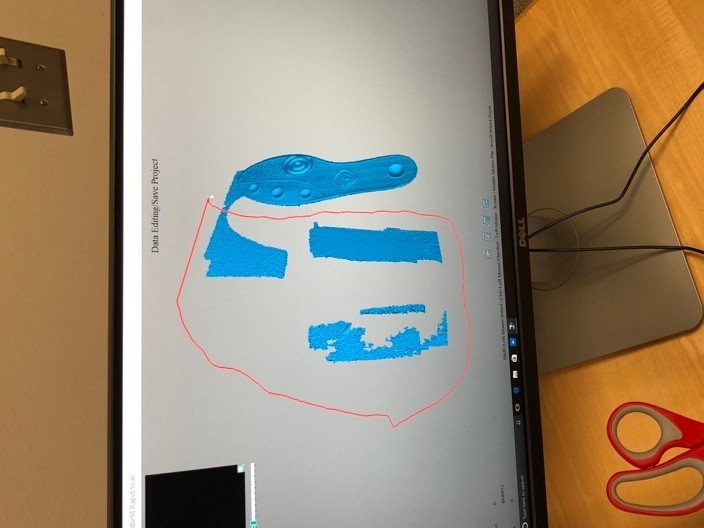
\includegraphics[scale=.75, angle=270]{3D_Crop}
\caption{Select the portions of the scan that do not include the sole of the shoe.}
\label{Image 6}
\end{figure}

\begin{figure}[!htp]
\centering
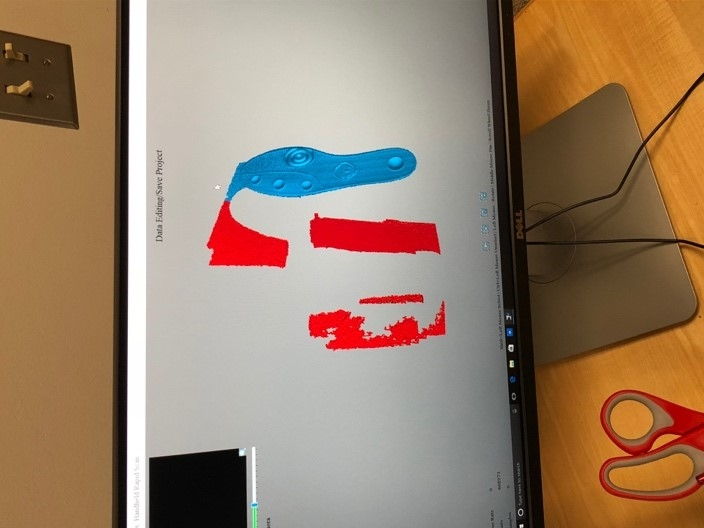
\includegraphics[scale=.75, angle=270]{3D_Crop_2}
\caption{The selected portions will turn red.}
\label{Image 7}
\end{figure}

\newpage

9. Use the trash scan icon included on the bottom tool bar to delete unwanted portions of the scan (Figure 8). The Final scan will resemble that in figure 9.

\begin{figure}[!htp]
\centering
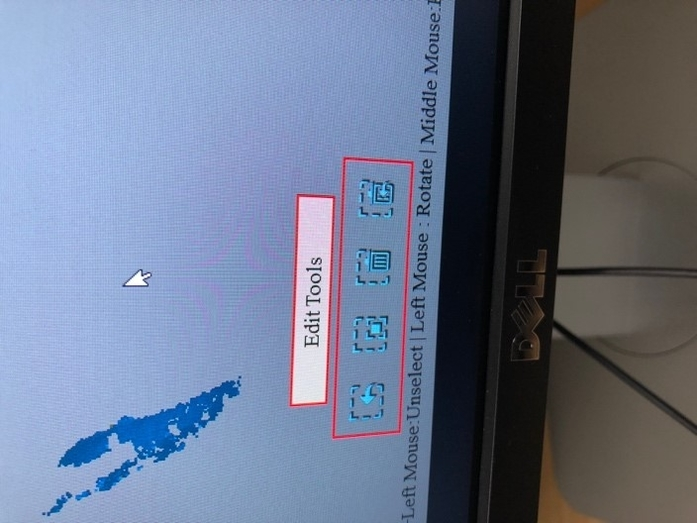
\includegraphics[scale=1, angle=270]{3D_Tools}
\caption{Select the delete button at the bottom of the screen to remove unwanted material in the scan. }
\label{Image 8}
\end{figure}

\begin{figure}[!htp]
\centering
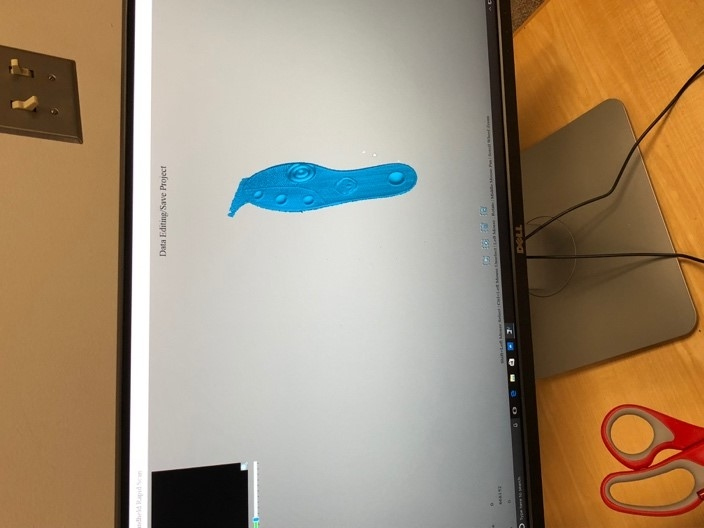
\includegraphics[scale=.75, angle=270]{3D_Cropped}
\caption{Sample of a final, cropped image}
\label{img:Finish2}
\end{figure}

\newpage

10. Select Finish Scan on the right tool-bar (Figure 10). Observe scan and determine if you need to continue scan to collect additional points and repeat steps 5-8. If you have collected all of the detail possible, select the Create Model icon (Figure 11).

\begin{figure}[!htp]
\centering
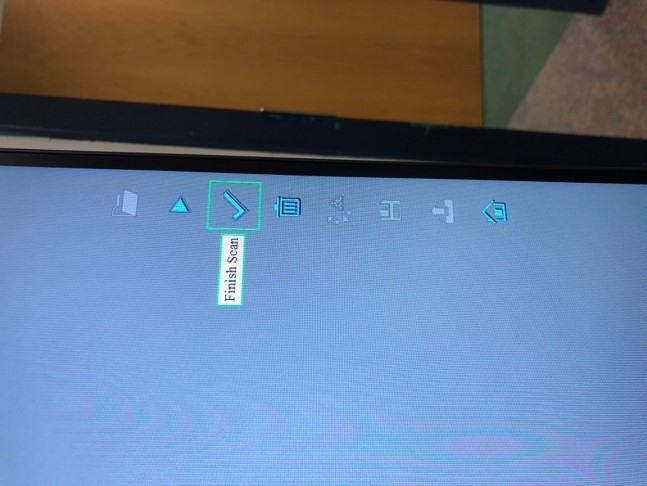
\includegraphics[scale=.75, angle=270]{3D_Finalize}
\caption{The "check mark" icon on the right tool-bar finalizes the image.}
\label{Image 10}
\end{figure}

\begin{figure}[!htp]
\centering
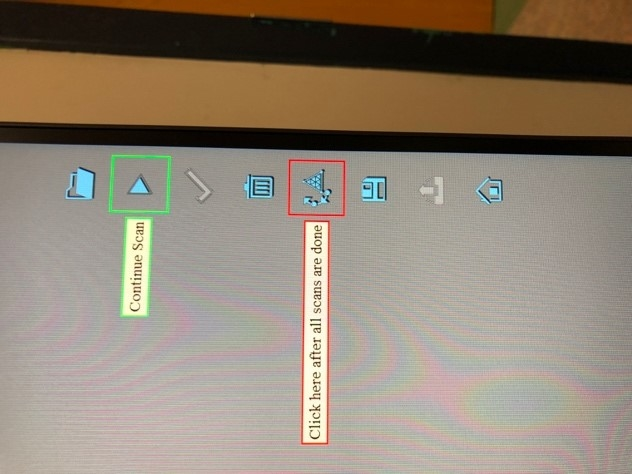
\includegraphics[scale=.75, angle=270]{3D_Finalize_2}
\caption{Begin final processing.}
\label{Image 11}
\end{figure}

\newpage

11.Select "Unwatertight Model" (Figure 12)

\begin{figure}[!htp]
\centering
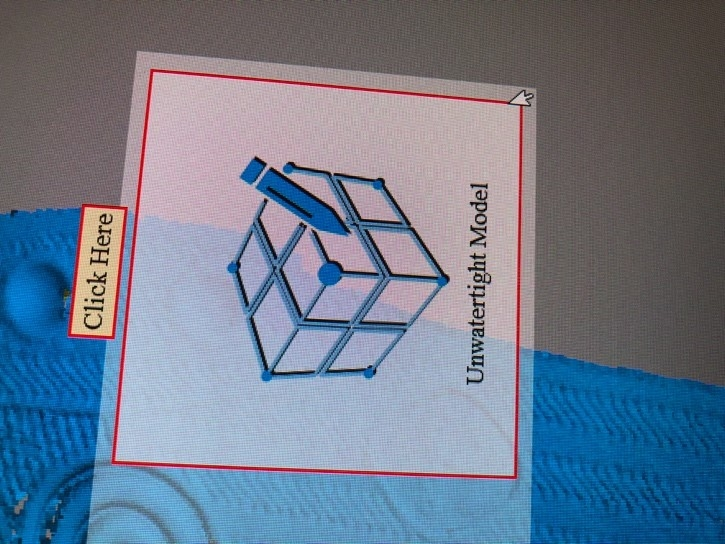
\includegraphics[scale=1, angle=270]{3D_Unwatered}
\caption{Select "Unwatertight Model". }
\label{Image 12}
\end{figure}



12. A small screen will come up following model selection. Make sure they all match those in figure 13.

\begin{figure}[!htp]
\centering
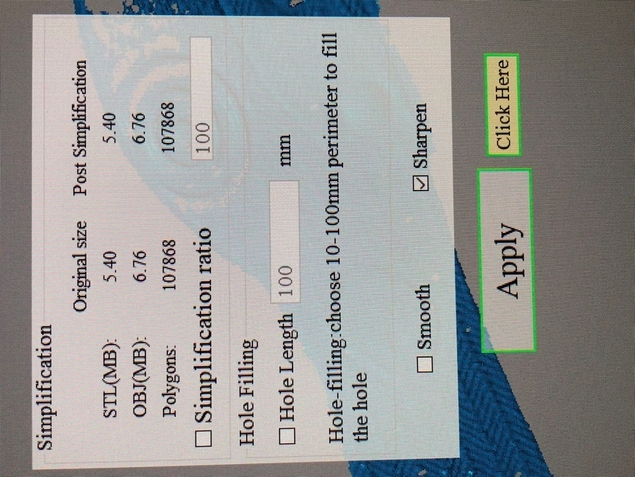
\includegraphics[scale=1, angle=270]{3D_End}
\caption{Apply the settings in the image below. }
\label{img:Apply}
\end{figure}

\newpage

13. Select save from the right hand toolbar making sure to select .stl as the file type when naming.

14. Select scale image.

\textbf{Note: Make sure that all images are saved in the correct drawer/file/directory
/digital file.}
\end{document}

